\documentclass{article}

\usepackage{graphicx}
\usepackage{tikz}
\usepackage{tikzsymbols}
\usetikzlibrary{calc,patterns,shapes.geometric}
\pagestyle{empty}
\usepackage[margin=0pt]{geometry}
\geometry{papersize={14in,12in}}

\def\centerarc[#1](#2)(#3:#4:#5){\draw[#1] ($(#2)+({#5*cos(#3)},{#5*sin(#3)})$) arc (#3:#4:#5);}

\begin{document}
	\begin{figure}
		\centering
		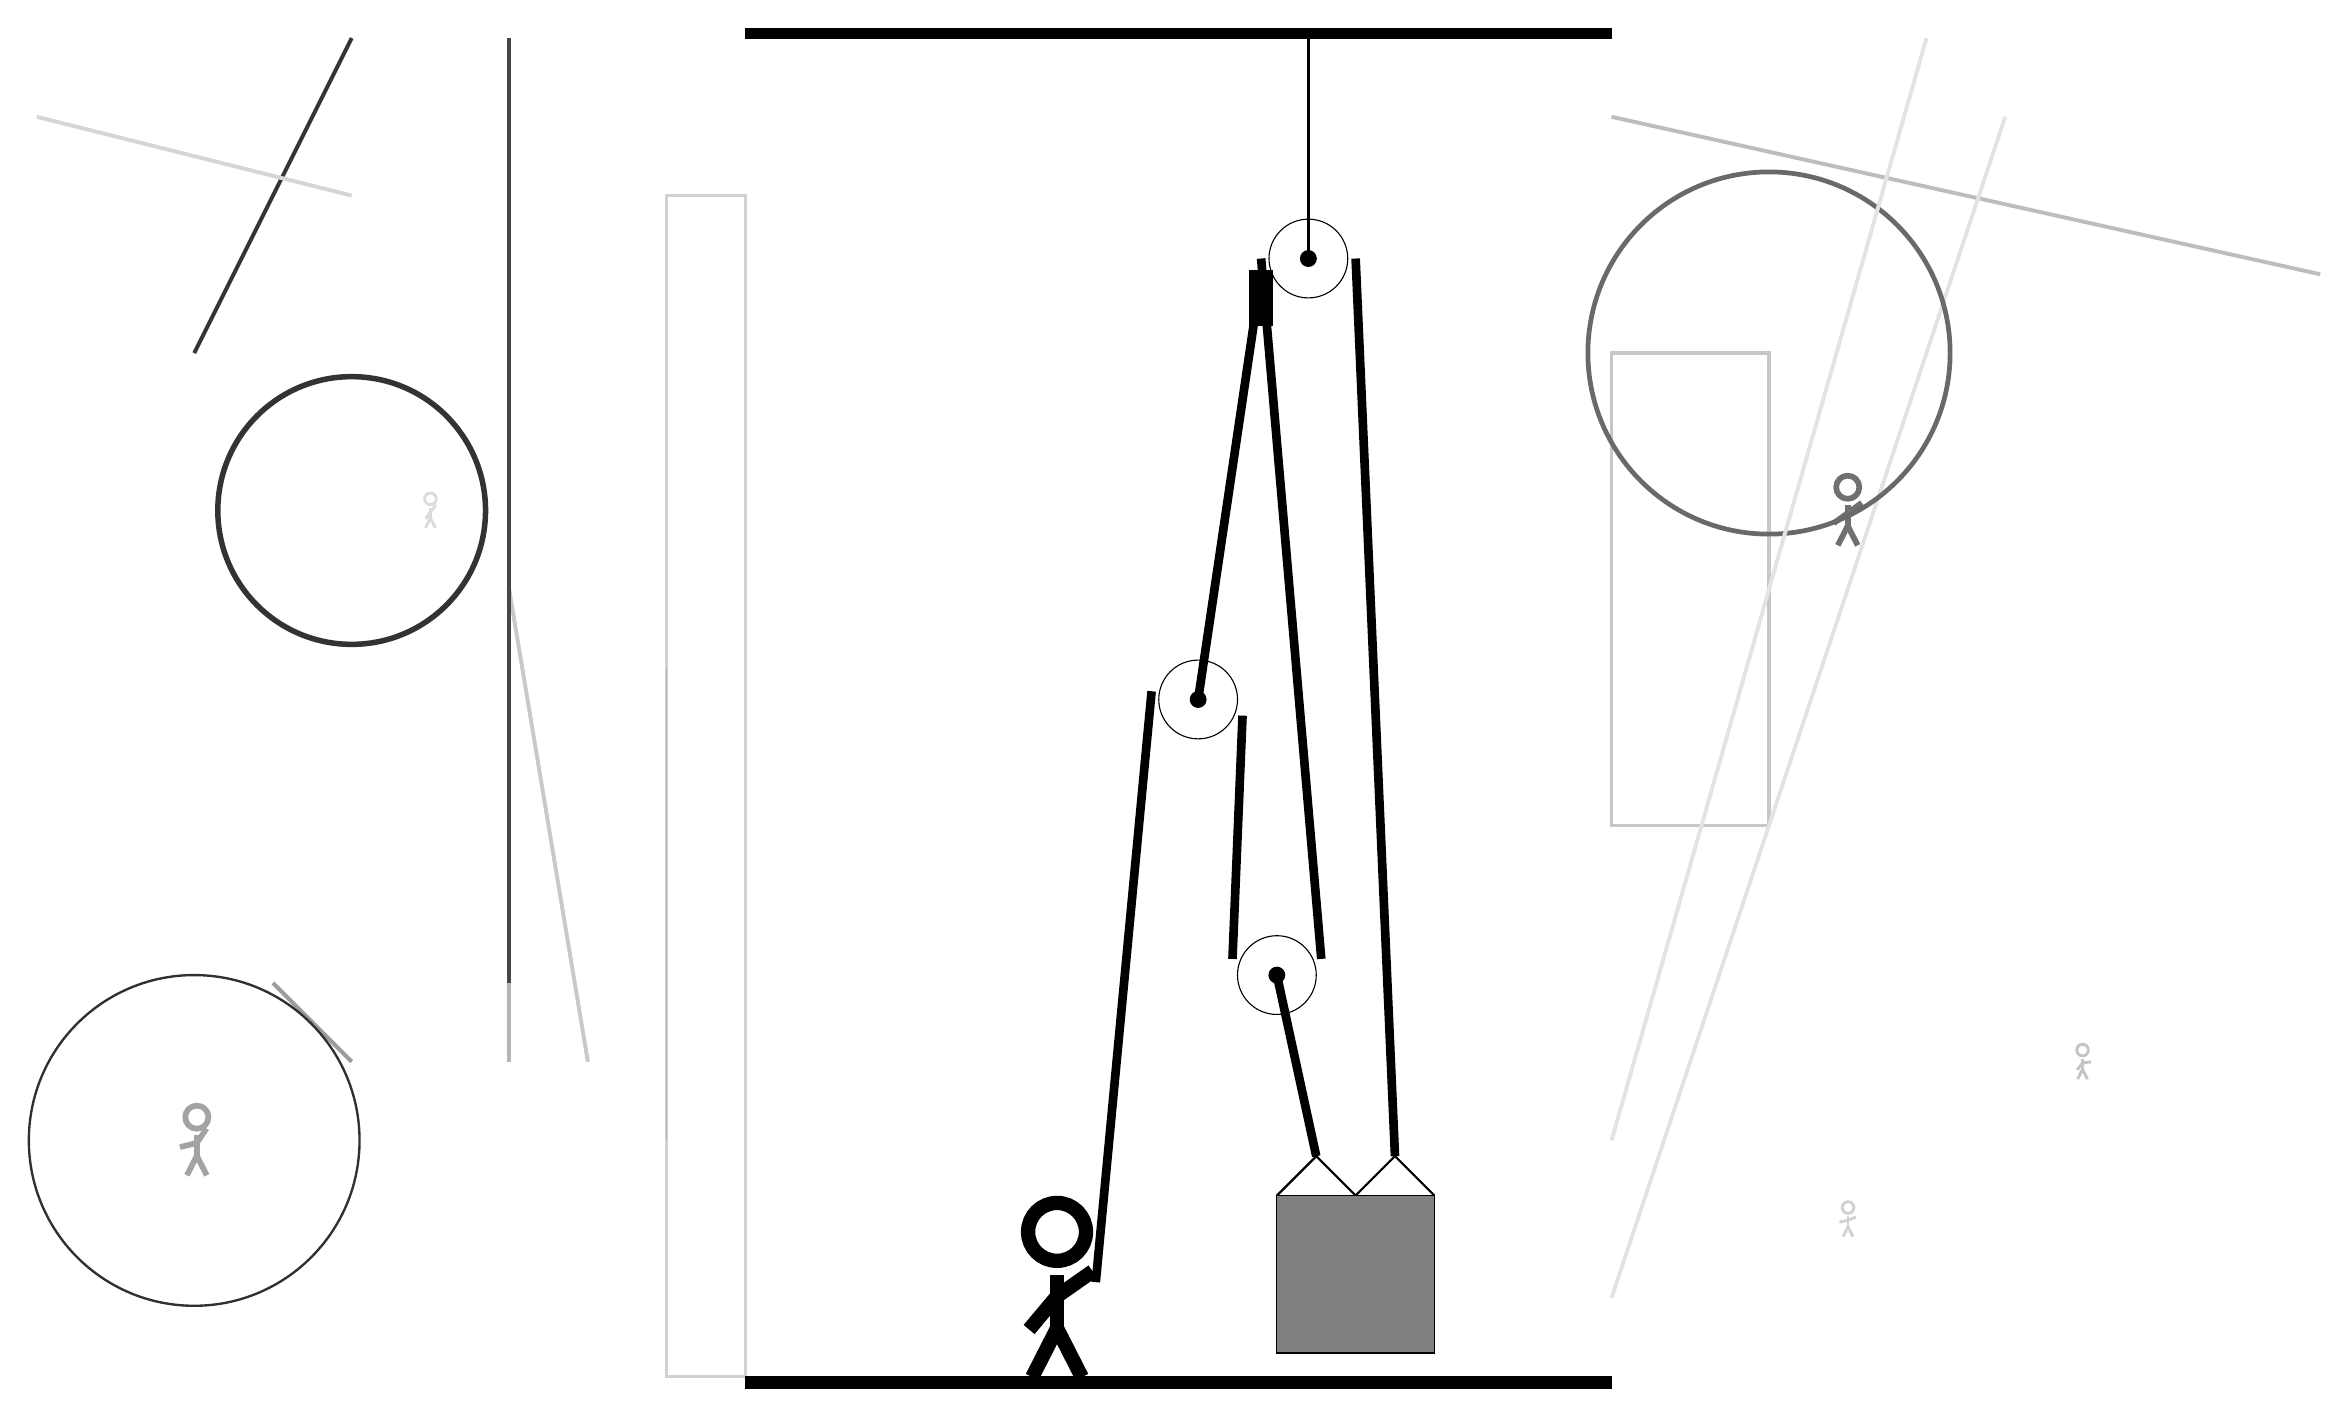
\begin{tikzpicture}
			%%%%% START %%%%%
			
			\draw[fill=black] (-6, 14) rectangle (5, 14.125);
			
			\draw (-0.25, 5.6) circle (0.5);
			\draw[fill=black] (-0.25, 5.6) circle (0.1);
			
			\draw (0.75, 2.1) circle (0.5);
			\draw[fill=black] (0.75, 2.1) circle (0.1);
			
			\draw (1.15, 11.2) circle (0.5);
			\draw[fill=black] (1.15, 11.2) circle (0.1);
			\draw[very thick] (1.15, 11.2) -- (1.15, 14);
			
			\draw [line width=0.7mm, color=black!14](-9, 9) circle (0.0);
			
			\node[line width=0.5mm, color=black!14] at (-10, 8) {\Strichmaxerl[2][57][50]};
			\draw[line width=0.5mm, color=black!39](-11, 1) -- (-12, 2);
			\draw[line width=0.5mm, color=black!26](5, 13) -- (14, 11);
			
			\node[line width=0.6mm, color=black!36] at (-13, 0) {\Strichmaxerl[4][14][56]};
			\draw[line width=0.4mm, color=black!22] (5, 10) rectangle (7, 4);
			\draw[line width=0.5mm, color=black!29](-9, 1) -- (-9, 9);
			
			\draw [line width=0.7mm, color=black!80](-11, 8) circle (1.7);
			\node[line width=0.6mm, color=black!18] at (8, -1) {\Strichmaxerl[2][10][23]};
			\draw[line width=0.4mm, color=black!18] (-6, -3) rectangle (-7, 12);
			
			\draw [line width=0.3mm, color=black!81](-13, 0) circle (2.1);
			\draw[line width=0.5mm, color=black!21](-8, 1) -- (-9, 7);
			\node[line width=0.3mm, color=black!23] at (11, 1) {\Strichmaxerl[2][52][7]};
			
			\draw[line width=0.5mm, color=black!11](5, -2) -- (10, 13);
			\draw[line width=0.5mm, color=black!79](-11, 14) -- (-13, 10);
			\node[line width=0.5mm, color=black!56] at (8, 8) {\Strichmaxerl[4][36][36]};
			
			\draw [line width=0.6mm, color=black!59](7, 10) circle (2.3);
			
			\draw[line width=0.2mm, color=black!27] (-7, 6) rectangle (-7, 0);
			\draw[line width=0.5mm, color=black!16](-11, 12) -- (-15, 13);
			
			\draw[line width=0.5mm, color=black!72](-9, 14) -- (-9, 2);
			\draw[line width=0.5mm, color=black!11](9, 14) -- (5, 0);
			
			
			\draw[thick]  (0.75, -0.7) -- (1.25, -0.2) -- (1.75, -0.7) -- (2.25, -0.2) -- (2.75, -0.7);
			\draw[fill=black!50] (0.75, -0.7) rectangle (2.75, -2.7);
			
			\draw[line width=1.1mm] (-0.25, 5.6) -- (0.55, 11.0);
			\draw[line width=1.1mm, fill=black](0.45, 10.4) rectangle (0.65, 11.0);
			\draw[line width=1.1mm] (-1.55, -1.8) -- (-0.8409, 5.7042);
			\centerarc[line width=1.1mm](-0.25, 5.6)(-20:170:0.6);
			\draw[line width=1.1mm] (0.3138, 5.3948) -- (0.1862, 2.3052);
			\centerarc[line width=1.1mm](0.75, 2.1)(160:380:0.6);
			\draw[line width=1.1mm] (1.3138, 2.3052) -- (0.55, 11.2);
			\draw[line width=1.1mm](0.75, 2.1) -- (1.25, -0.2);
			\centerarc[line width=1.1mm](1.15, 11.2)(0:180:0.6);
			\draw[line width=1.1mm] (1.75, 11.2) -- (2.25, -0.2);
			
			\node at (-2, -1.9) {\Strichmaxerl[10][50][35]};
			
			\draw[fill=black] (-6, -3) rectangle (5, -3.15);
			
			%%%%% END %%%%%
		\end{tikzpicture}
	\end{figure}	
\end{document}